\documentclass[a4paper, 12pt]{article}
\usepackage[total={17cm,25cm}, top=2.5cm, left=2.5cm, right=2.5cm,  includefoot]{geometry}
\usepackage[utf8]{inputenc}
\usepackage{array}
\usepackage{multirow}
\usepackage{hhline}
\usepackage{gensymb}
\usepackage{graphicx}
\graphicspath{ {} }
\usepackage[czech]{babel}
\usepackage{enumitem}
\usepackage{pdfpages}
\usepackage{amsmath}
\usepackage{verbatim}
\usepackage{listings}
\usepackage{hyperref}
\usepackage{amssymb}


\pagestyle{empty} % vypne číslování stránek




\usepackage[OT2,OT1]{fontenc}
\newcommand\cyr
{
\renewcommand\rmdefault{wncyr}
\renewcommand\sfdefault{wncyss}
\renewcommand\encodingdefault{OT2}
\normalfont
\selectfont
}
\DeclareTextFontCommand{\textcyr}{\cyr}
\def\cprime{\char"7E }
\def\cdprime{\char"7F }
\def\eoborotnoye{\char’013}
\def\Eoborotnoye{\char’003}


\begin{document}



\begin{titlepage}
\begin{center}
\noindent
\Large \textbf{České vysoké učení technické v Praze }\\ Fakulta stavební
\vspace{5cm}

\huge

%vložení loga cvut
\begin{figure}[h!]
	\centering
	
\includegraphics[width=7cm]{logo.png}
\end{figure}

\vspace{0.5cm}

Algoritmy v digitální kartografii \\

\vspace{3cm}

\Huge  
Digitální model terénu a jeho analýzy\\

\vspace{2cm}

\Large
Bc. Petra Pasovská \\
Bc. David Zahradník \\

\end{center}

\end{titlepage}




\pagestyle{plain}     % zapne obyčejné číslování
\setcounter{page}{1}  % nastaví čítač stránek znovu od jedné

\tableofcontents
\newpage

\section{Zadání}
Níže uvedené zadání je kopie ze stránek předmětu. 

\begin{figure}[h!]
	\centering
	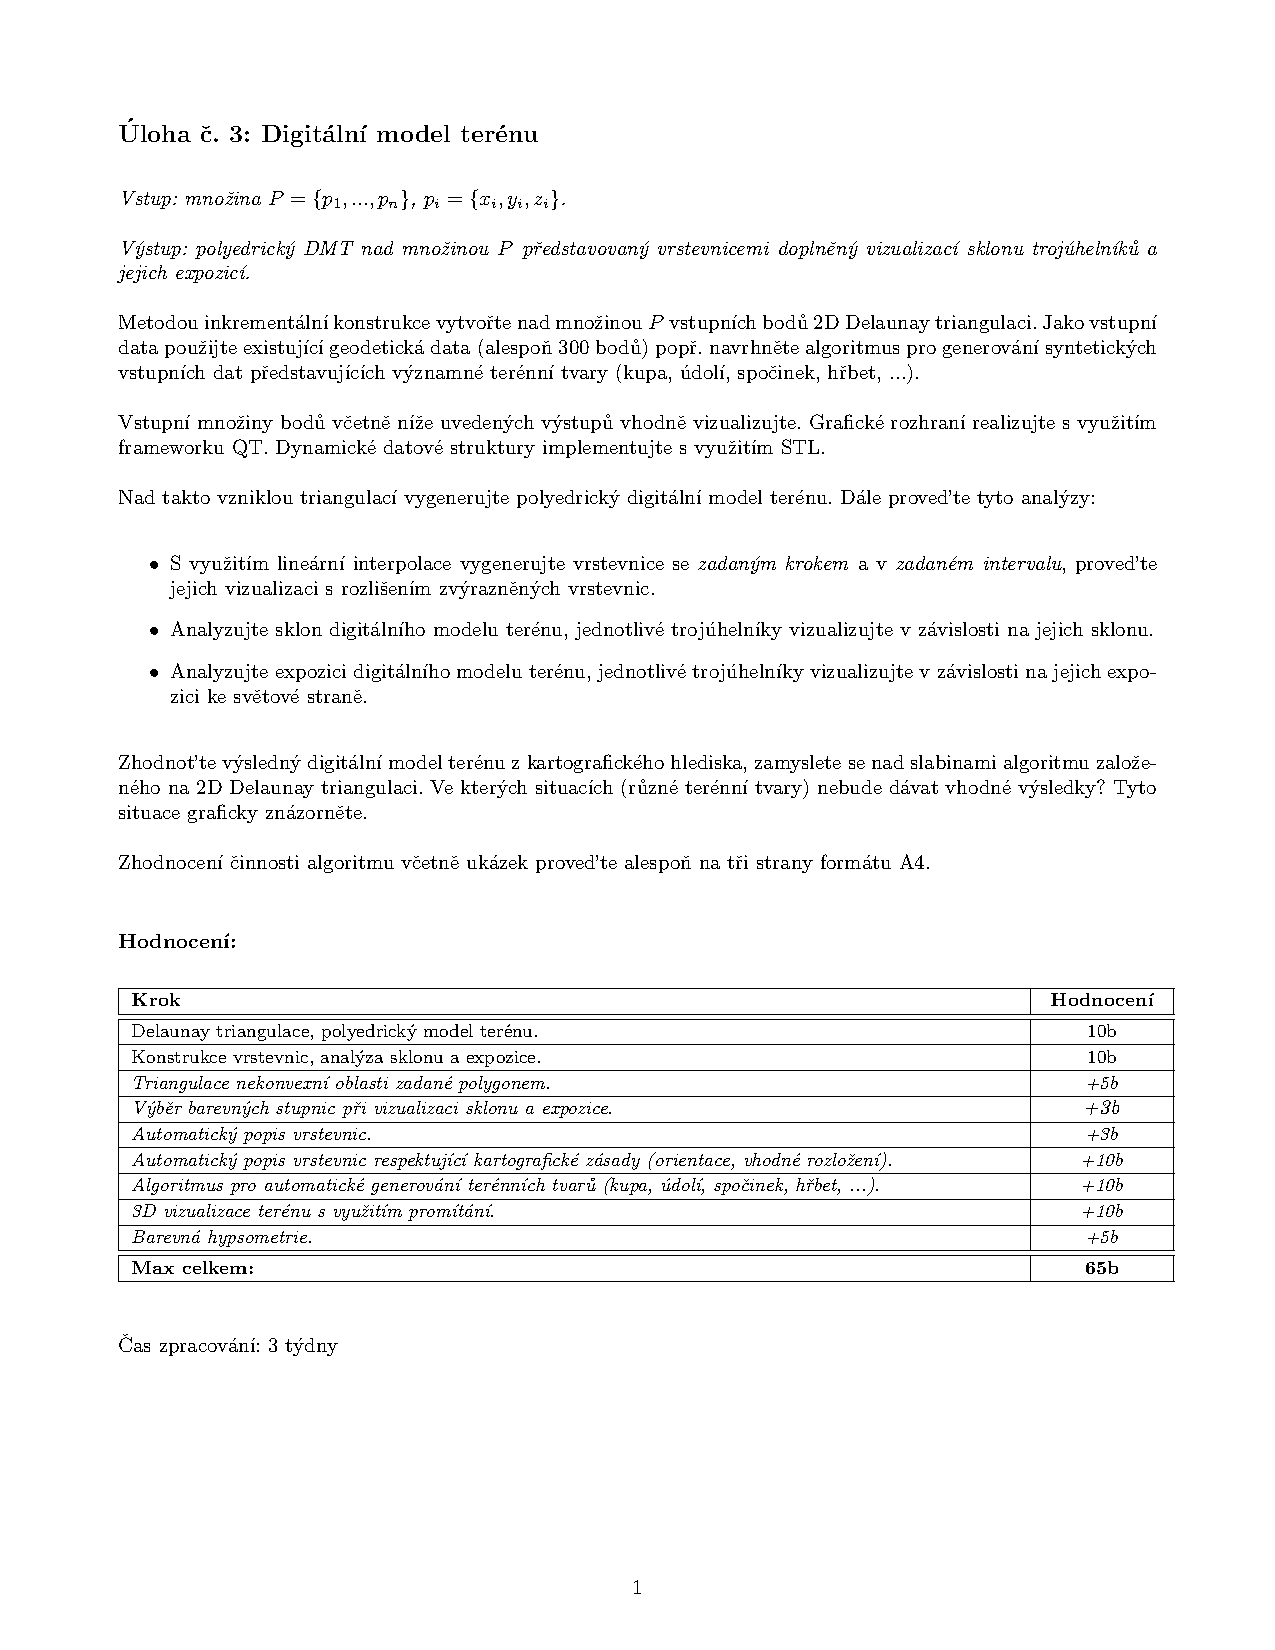
\includegraphics[clip, trim=0cm 10cm 0cm 3cm, width=1.2\textwidth]{zadani.pdf}
\end{figure}

\subsection{Údaje o bonusových úlohách}
Nebyly vytvořeny žádné bonusové úlohy.


\clearpage

\section{Popis a rozbor problému}
Hlavním cílem této úlohy je tvorba aplikace, která nad výškopisnými body vytvoří Delaunay triangulaci, vrstevnice a vypočte sklon a expozici k světovým stranám.\\
\\
Obecně triangulační algoritmy jsou nejvíce zkoumané algoritmy digitální kartografie v dnešní době. Slouží k různým účelům např. tvorba digitálního modelu terénu, plánování pohybu robotů, detekce otisků prstů.  [Zdroj: 1]
\\


\section{Popis použitých algoritmů}
Existuje několik způsobů jak vytvořit triangulaci s různými kritérii. V této úloze jsme ze zabývali Delaunay triangulací pomocí metody inkrementální konstrukce.

\subsection{Delaunay triangulací}
Delaunay triangulace je nejčastěji používanou trianglucí při tvorbě digitálního modelu terénu. Delaunay triagulaci lze provádět v rovině i v prostoru.
\\
\subsubsection{Vlastnosti}
Uvnitř opsané kružnice libovolného trojúhelníku triangulace neleží žádný jiný bod.
\\
Maximalizuje minimální úhlel, avšak neminimalizuje maximální úhle v trojúhelníku.
\\
Vůči kritériu minimálního úhlu je lokálně i globálně optimální.
\\
Triangulace je jednoznáčná pokud čtyři body neleží na kružnici.
\\

Triangulace byla realizována pomocí metody inkrementální konstrukce. Tento algoritmus je založen na postupném hledání bodu, který k bodům hrany tvoří minimální opsanou kružnici. Každá hrana je orientovaná a bod se hledá pouze v její levé polorovině.\\
Je-li nalezen bod s výše uvedeným kritériem vytvoří se dvě nové hrany, které jsou přidány do triangulace. Nenalezne-li se daný bod, prohodí se orientace hrany a hledání pokračuje.\\
Hrany, které nebyly zlegalizovány (nebyl k ní ještě nalezen třetí bod), jsou ukládány do struktury Active Edge List (AEL). Pokud k dané hraně byl nalezen tří bod, hrana se ze struktury odstraní. Než je hrana vložena do struktury, kontroluje se zda hrana už ve struktuře není s opačnou orientací, pokud je, hrana se nevloží. Algoritmus běží dokud struktura AEL není prázdná.

\subsubsection{Implementace metody}
\begin{enumerate}
\item Nalezení pivota q a k němu nejbližší bod:  $ q = min(y_i) $ 
\item Hledání prvního Delaunay bodu.
\item Vytvoření prvního Delaunay trojúhelníku.
\item Hrany trojúhelníka se uloží do triangulace a do AEL.
\item Dokud není AEL prázdný proveď.
\subitem Hledej Delaunay bod k hraně z AEL.
\subitem Pokud Delaunay bod existuje.
\subsubitem Přidej nové hrany do DT.
\subsubitem Pokud nová hrana není v AEL přidej.
\end{enumerate}

\subsection{Vrstevnice}
V úloze byly vrstevnice konstruovány lineární interpolací. U lineární interpolace je rozestup vrstevnice mezi dvěma body konstantní, tedy i spád. Při konstrukci vrstevnic hledáme průsečnici vodorovné roviny o výšce Z a rovinu trojúhelníka triangulace.\\

\subsubsection{Implementace metody}
\begin{enumerate}
\item Pro všechny hrany triangulace:
\subitem Otestuj zda hrana protíná vodorovnou rovinu o výšce Z:
\subitem Pokud protíná spočti polohové souřadnice.
\subitem Vytvoř hranu tvořící vrstevnici.

\end{enumerate}

\subsection{Sklon terénu}
Skon terénu je definován jako úhle mezi normálovým vektorem (0,0,1) a normálovým vektorem roviny trojúhelníku.

\subsubsection{Implementace metody}
\begin{enumerate}
\item Pro všechny trojúhelníky triangulace:
\subitem Vypočti sklon:
\end{enumerate}

\subsection{Expozice terénu}
Expozice terénu je definována jako azimut k průmětu normálového vektoru roviny trojúhelníka do roviny x,y.

\subsubsection{Implementace metody}
\begin{enumerate}
\item Pro všechny trojúhelníky triangulace:
\subitem Vypočti expozici:
\end{enumerate}

\section{Informace o bonusových úlohách}


\section{Vstupní data}
\\

\section{Výstupní data}
\\


\clearpage
\section{Aplikace}
\begin{figure}[h!]
	\centering
	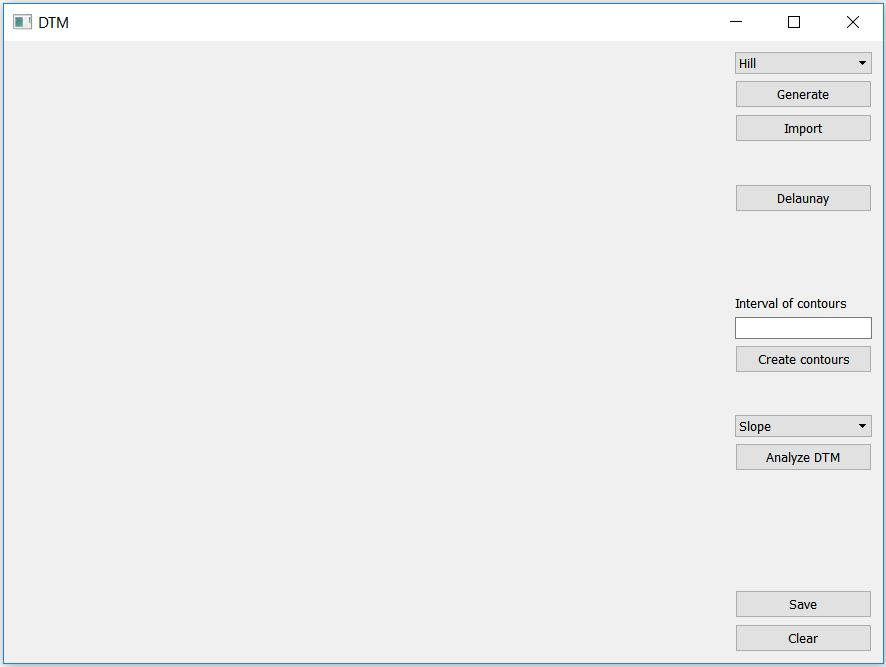
\includegraphics[width=10cm]{vstup.jpg}
	\caption{Zobrazené okno po spuštění aplikace}
\end{figure}

\begin{figure}[h!]
	\centering
	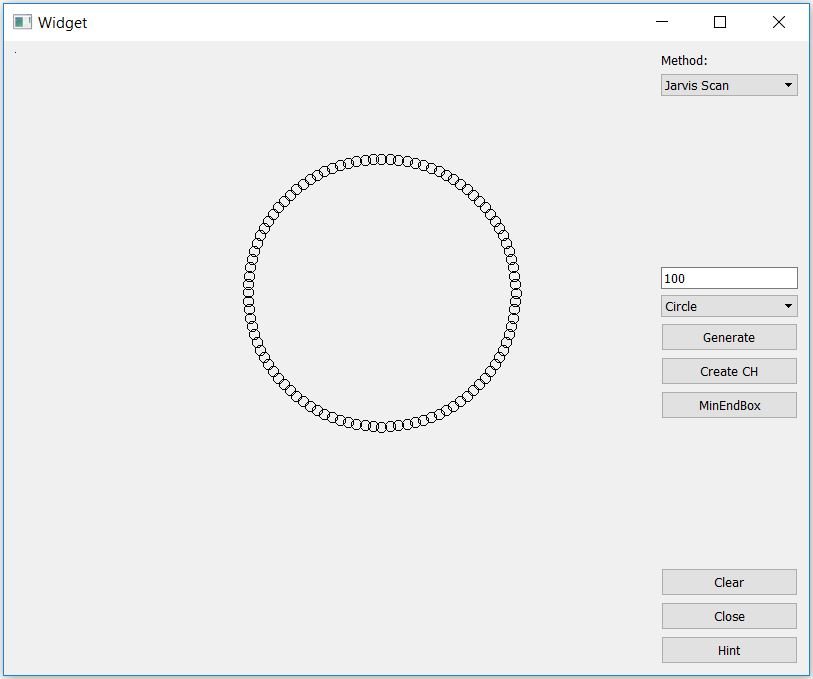
\includegraphics[width=10cm]{circle.jpg}
	\caption{Vygenerované body v kruhu}
\end{figure}

\begin{figure}[h!]
	\centering
	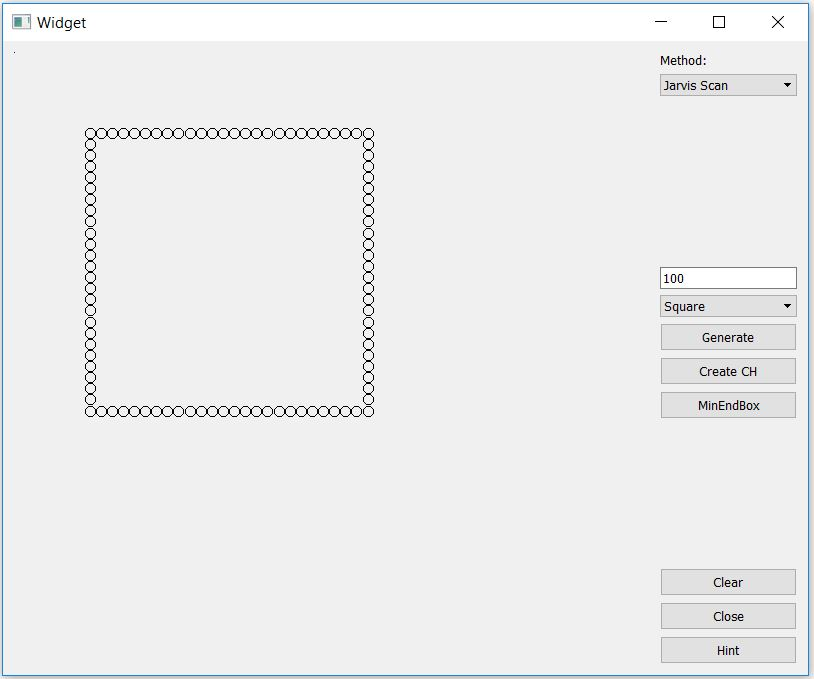
\includegraphics[width=10cm]{square.jpg}
	\caption{Vygenerované body ve čtverci}
\end{figure}

\begin{figure}[h!]
	\centering
	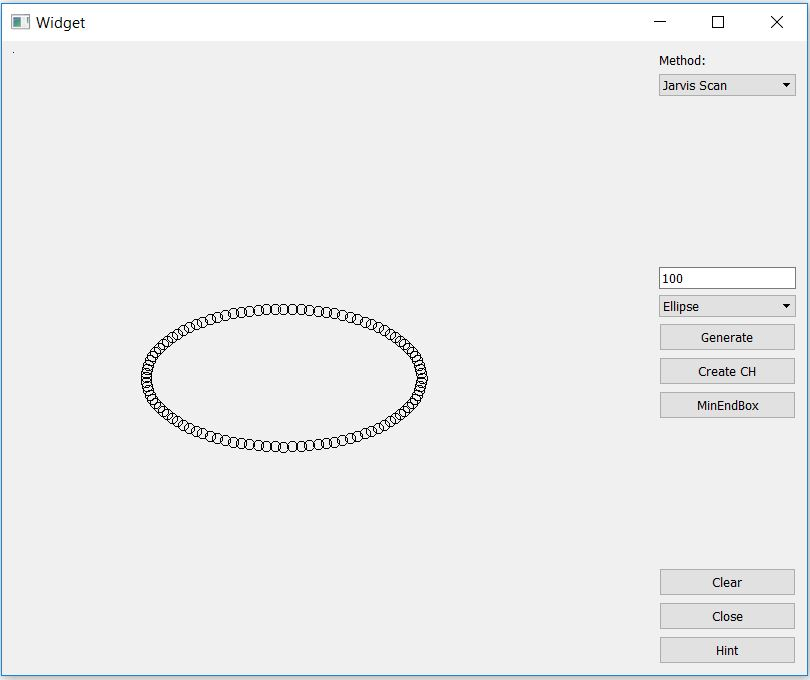
\includegraphics[width=10cm]{ellipse.jpg}
	\caption{Vygenerované body v elipse}
\end{figure}

\begin{figure}[h!]
	\centering
	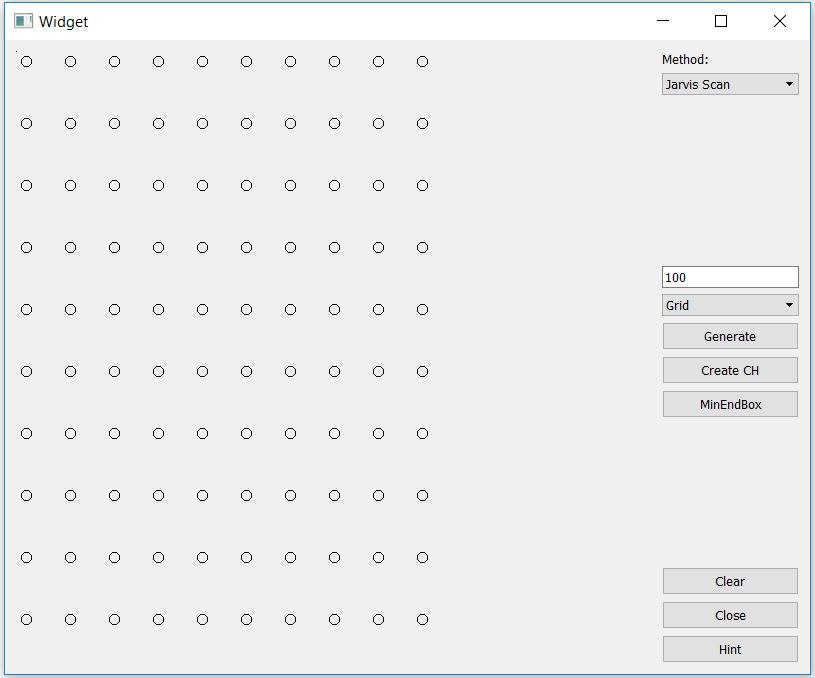
\includegraphics[width=10cm]{grid.jpg}
	\caption{Vygenerované body v pravidelné mřížce}
\end{figure}

\begin{figure}[h!]
	\centering
	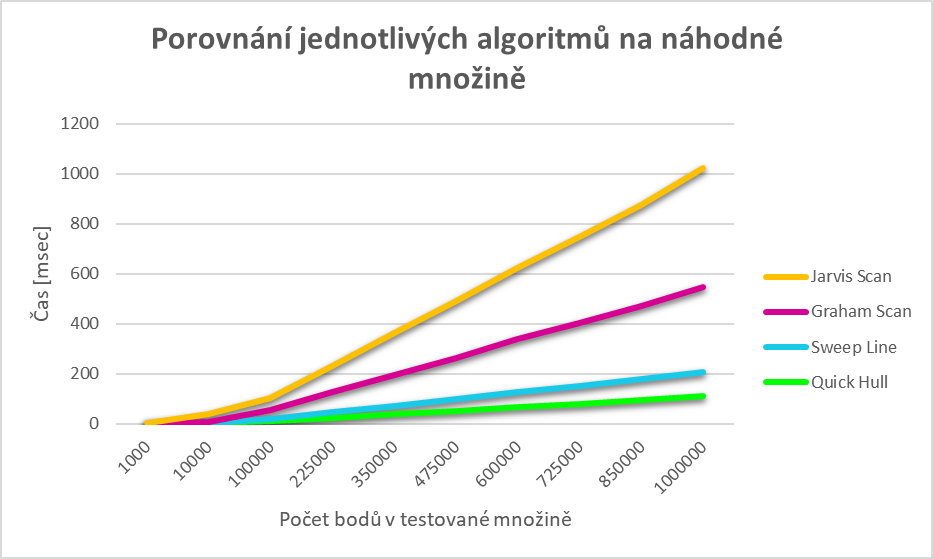
\includegraphics[width=10cm]{random.jpg}
	\caption{Náhodně vygenerované body}
\end{figure}

\begin{figure}[h!]
	\centering
	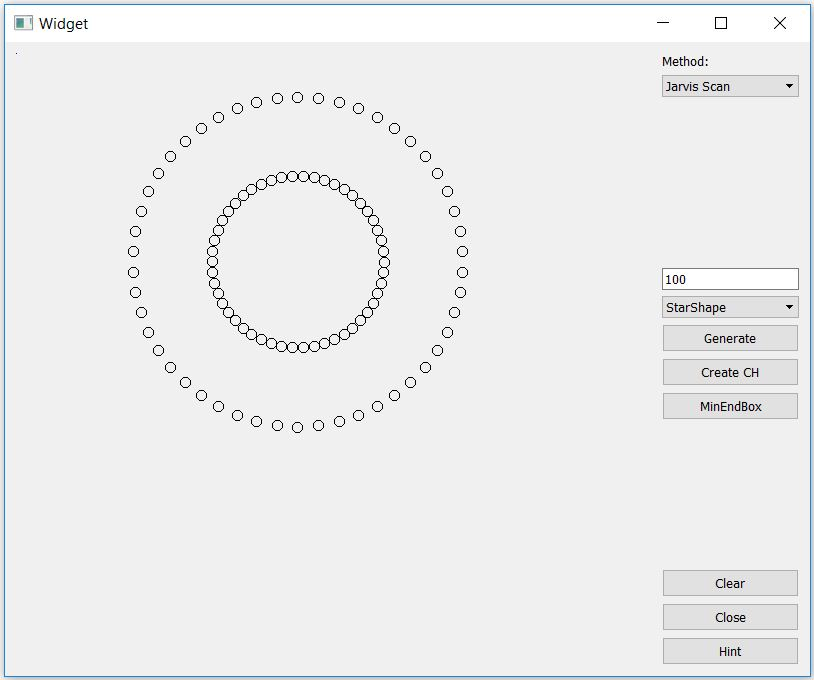
\includegraphics[width=10cm]{star_shaped.jpg}
	\caption{Vygenerované body ve tvaru Star Shaped}
\end{figure}

\begin{figure}[h!]
	\centering
	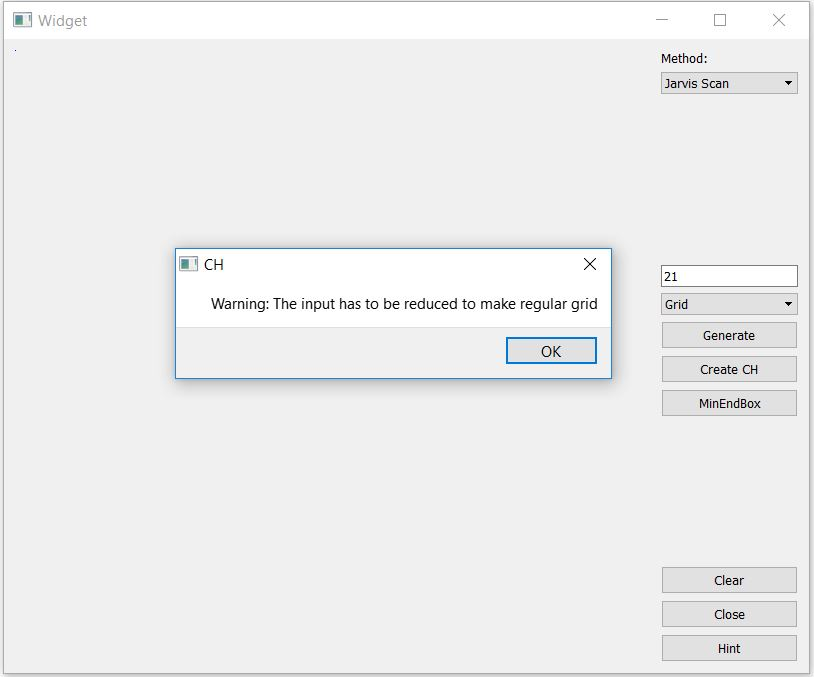
\includegraphics[width=10cm]{warning_grid.jpg}
	\caption{Varování na redukci vloženého počtu bodů při tvorbě gridu }
\end{figure}

\begin{figure}[h!]
	\centering
	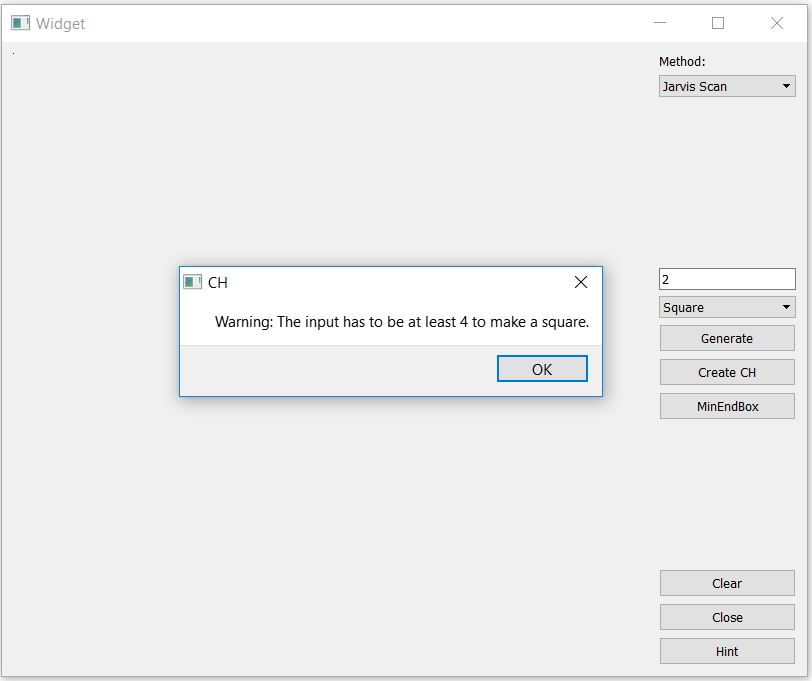
\includegraphics[width=10cm]{warning_square.jpg}
	\caption{Varování při neplatném vstupu při tvorbě čtverce}
\end{figure}

\begin{figure}[h!]
	\centering
	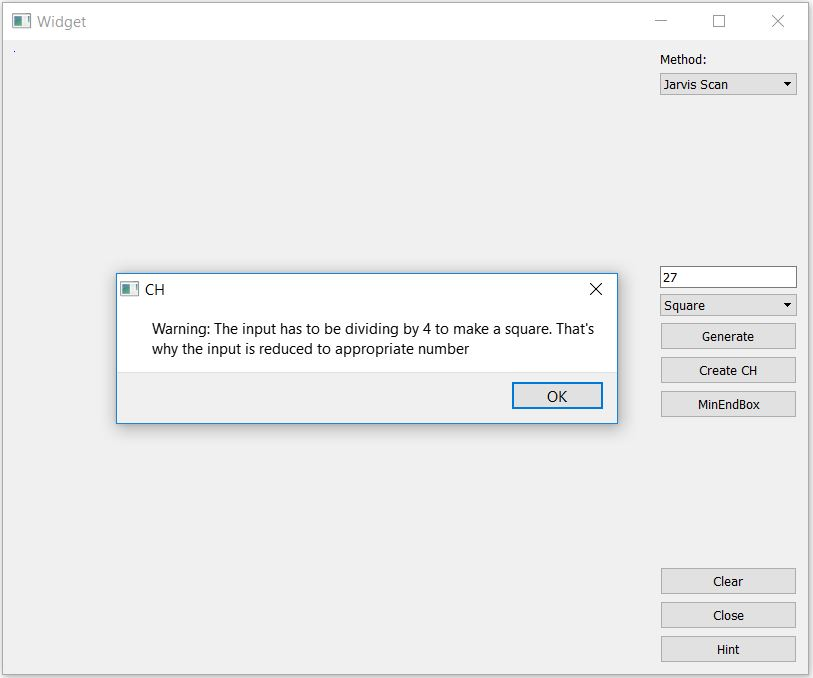
\includegraphics[width=10cm]{warning_square2.jpg}
	\caption{Varování na redukci vloženého počtu bodů při tvorbě čtverce}
\end{figure}

\begin{figure}[h!]
	\centering
	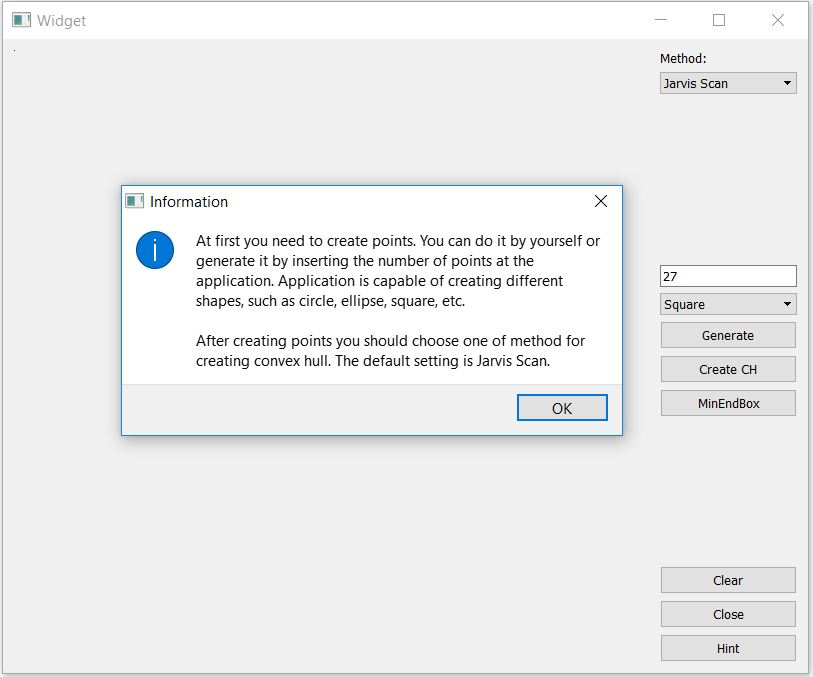
\includegraphics[width=10cm]{hint.jpg}
	\caption{Nápověda, pokud si uživatel nebude jistý, jak v aplikaci postupovat}
\end{figure}

\begin{figure}[h!]
	\centering
	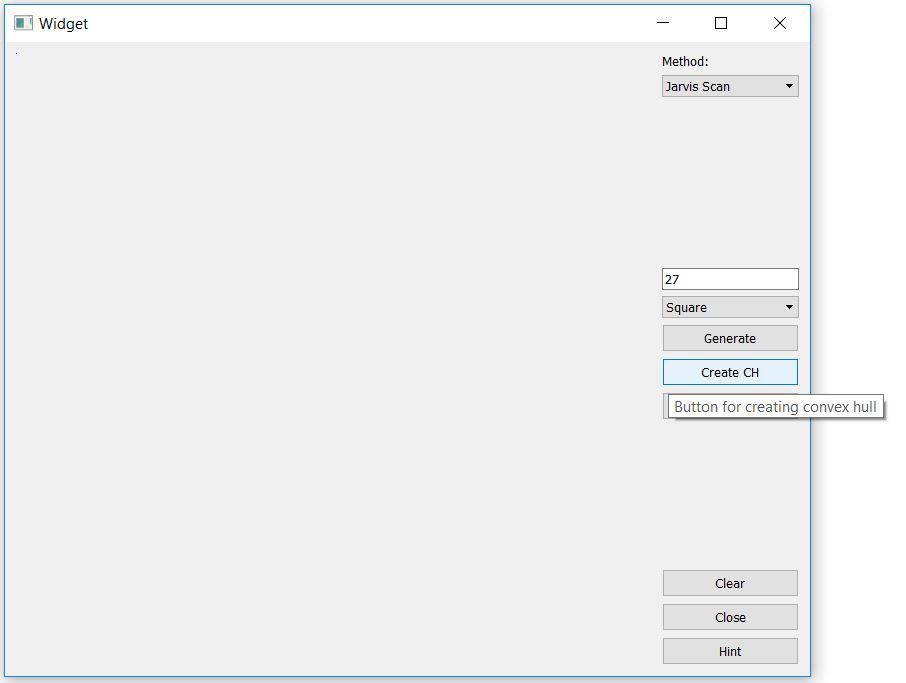
\includegraphics[width=10cm]{tooltip.jpg}
	\caption{Po přiložení kurzoru se zobrazí informace o objektu}
\end{figure}

\begin{figure}[h!]
	\centering
	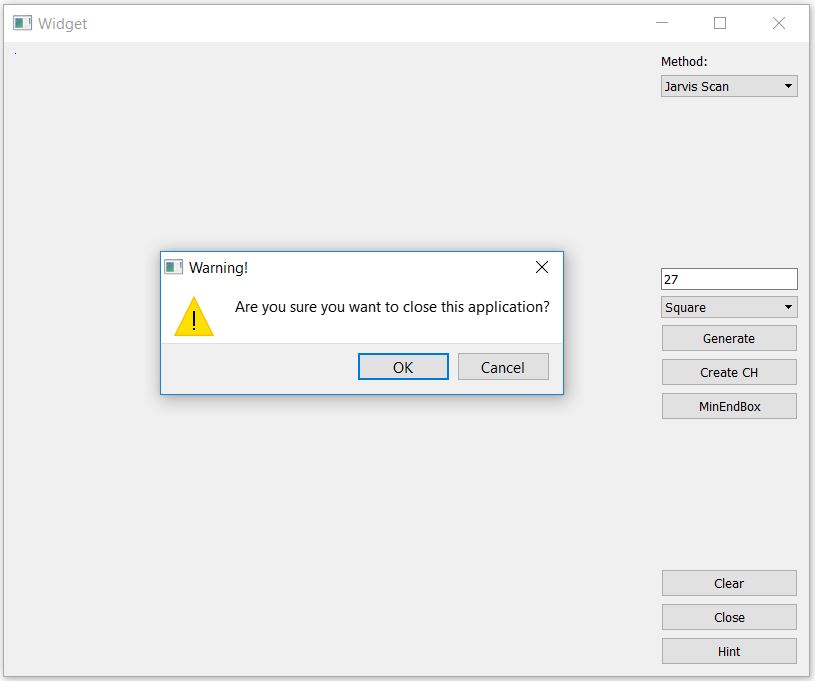
\includegraphics[width=10cm]{close.jpg}
	\caption{Vyskakovací okno při ukončování aplikace}
\end{figure}

\begin{figure}[h!]
	\centering
	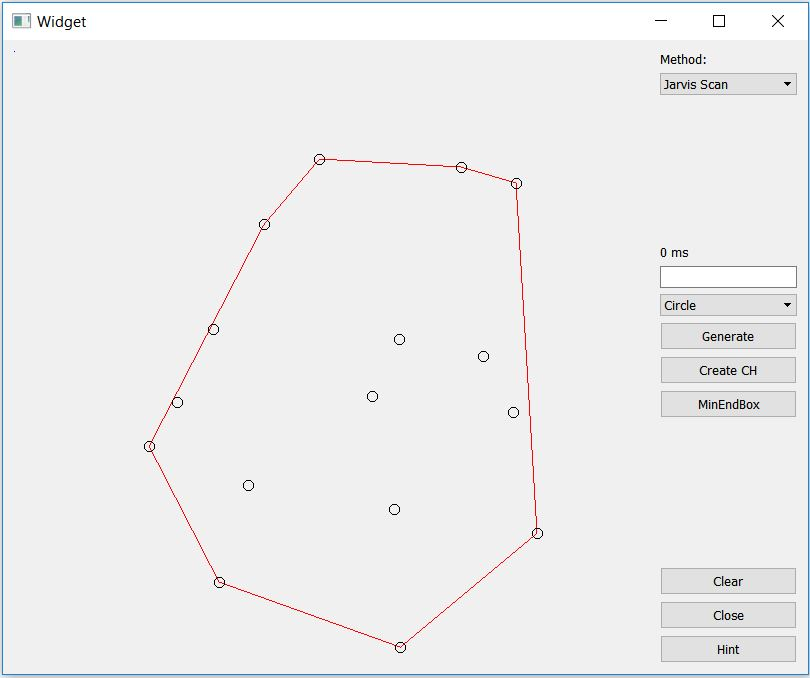
\includegraphics[width=10cm]{jarvis_ch.jpg}
	\caption{Tvorba konvexní obálky metodou Jarvis Scan}
\end{figure}

\begin{figure}[h!]
	\centering
	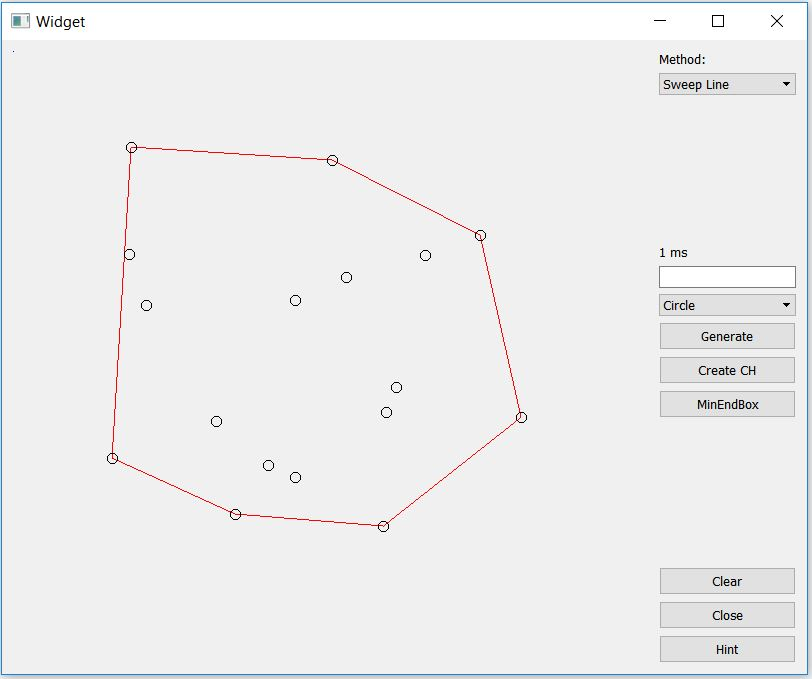
\includegraphics[width=10cm]{sweepline_ch.jpg}
	\caption{Tvorba konvexní obálky metodou Sweep Line}
\end{figure}

\begin{figure}[h!]
	\centering
	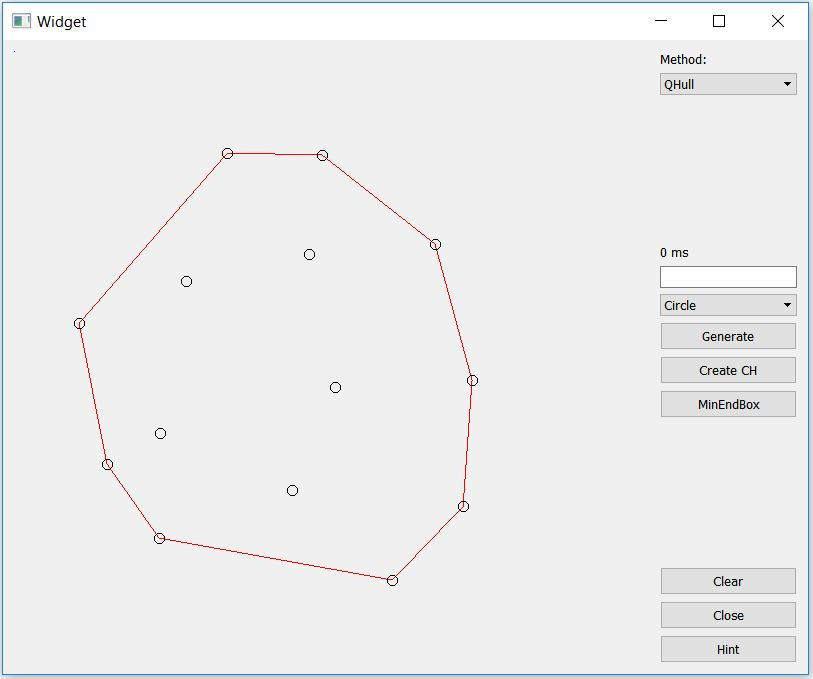
\includegraphics[width=10cm]{qhull_ch.jpg}
	\caption{Tvorba konvexní obálky metodou Quick Hull}
\end{figure}

\begin{figure}[h!]
	\centering
	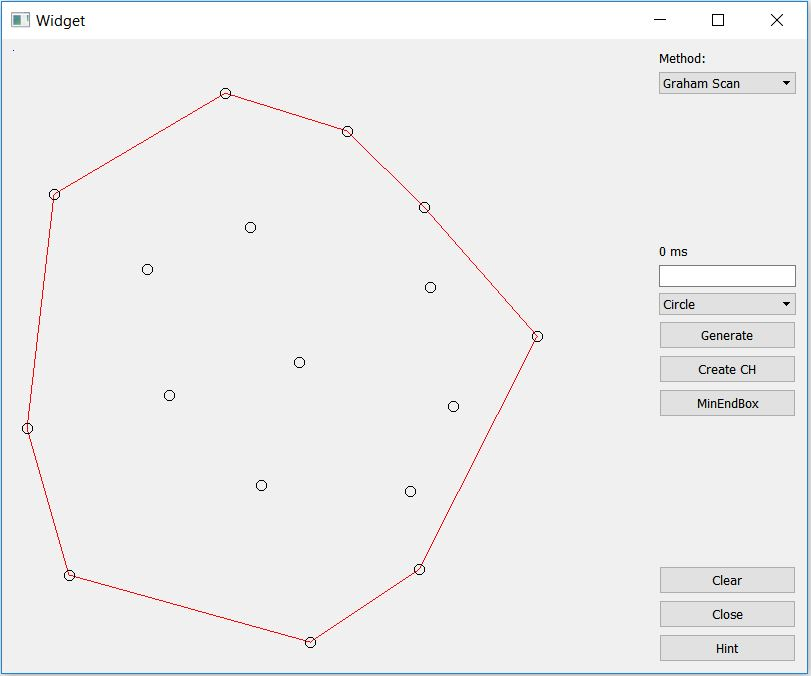
\includegraphics[width=10cm]{grahamscan_ch.jpg}
	\caption{Tvorba konvexní obálky metodou Graham Scan}
\end{figure}

\begin{figure}[h!]
	\centering
	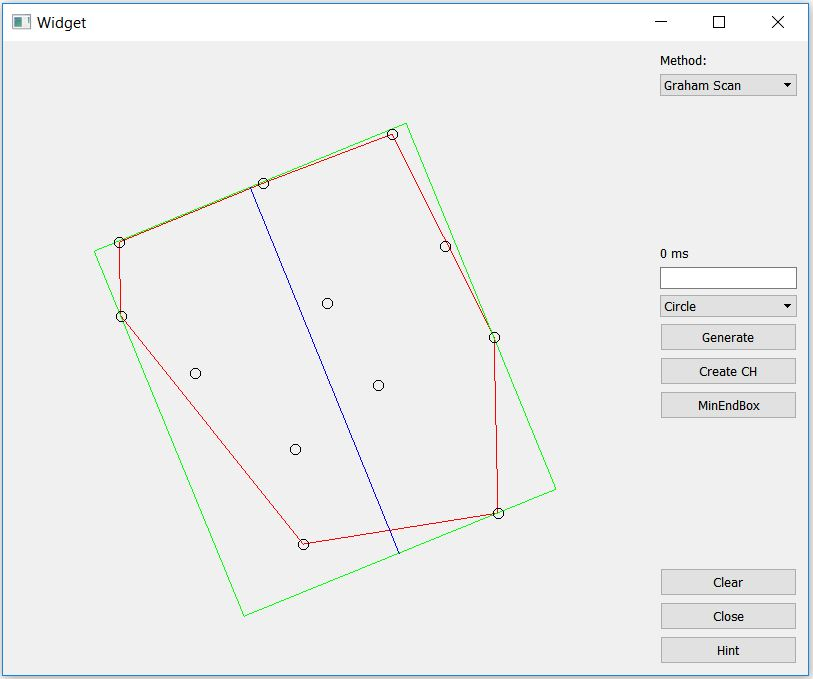
\includegraphics[width=10cm]{minBound.jpg}
	\caption{Tvorba minimálního ohraničujícího obdélníku}
\end{figure}

\clearpage

\section{Dokumentace}
\subsection{Třídy}
\subsubsection{Algorithms}
Třída Algorithms obsahuje několik metod. Metody jsou určeny pro výpočty použitých algoritmů.
\\

\textbf{double length2Points(QPoint q, QPoint p)}\\
Metoda, jejíž návratová hodnota je typu double, vrací velikost spojnice mezi dvěma body.
\\

\textbf{void polygonTransform(QPoint p, QPoint k, QPoint p1, QPoint k1, QPolygon \&pol)}\\
Metoda je přetížená pro  podobnostní transformaci QPolygon a QLine. Transformační klíč je dán dvěma body se souřadnicemi v obou souřadných soustavách. Body p a k jsou v souřadné soustavě, ze které pochází pol. Body p1 a k1 jsou v souřadné soustavě, do které chceme transformovat. Výsledek transformace se přeuloží do proměnné pol.
\\

\textbf{rotateByAngle(QPolygon \&points, double angle)}\\
Metoda je přetížená pro rotaci QPolygon a QLine. Prvky proměnné pol se pouze pootočí podle úhlu angle. Proměnná úhel je v radiánech. 
\\

\textbf{TPosition getPointLinePosition(QPoint \&q, QPoint \&a, QPoint \&b)}\\
Tato metoda slouží k určení pozice bodu q vůči linii tvořené body a, b. Výstupem metody je LEFT, RIGHT nebo ON.\\


\textbf{double get2LinesAngle(QPoint \&p1,QPoint \&p2,QPoint \&p3, QPoint \&p4)}\\
Pomocí této funkce je vypočítán úhel mezi dvěma přímkami, kde první přímka je tvořena body $ p_1 $ a $p_2$, druhá přímka je tvořena body $ p_3 $ a $p_4$.\\


\textbf{QPolygon CHJarvis (vector\textless QPoint \textgreater \&points)}\\
Metoda pro výpočet konvexní obálky nad vektorem bodů metodou Jarvis Scan. Metoda vrácí konvexní obálku s typem QPolygon.
\\

\textbf{QPolygon QHull (vector\textless QPoint \textgreater \&points)}\\
Metoda pro výpočet konvexní obálky nad vektorem bodů metodou Quick Hull. Metoda vrácí konvexní obálku s typem QPolygon.
\\

\textbf{void qh (int s, int e, vector\textless QPoint \textgreater \&p, QPolygon \&h)}\\
Pomocná metoda pro rekurzi v metodě Qhull. Na vstupu jsou indexy bodů s a e, které určují přímku, podle níž se určí, zda bod p patří do konvexní obálky H. Metoda nic nevrací, pouze ukládá body, které patří do konvexní obálky.
\\

\textbf{QPolygon GrahamScan (vector\textless QPoint \textgreater \&points)}\\
Metoda pro výpočet konvexní obálky nad vektorem bodů metodou Graham Scan. Metoda vrácí konvexní obálku s typem QPolygon.
\\

\textbf{QPolygon CHSweep (vector\textless QPoint \textgreater \&points)}\\
Metoda pro výpočet konvexní obálky nad vektorem bodů metodou Sweep Line. Metoda vrácí konvexní obálku s typem QPolygon.
\\

\textbf{void minimumAreaEnclosingBox (QPolygon \&ch, QPolygon \&rectangle, QLine \&direction)}\\
Metoda pro výpočet hlavních směrů budovy. Na vstupu je konvexní obálka ch a prázdné proměnné rectangle a direction. Do rectangle se uloží minimální ohraničující obdélník a do direction hlavní směr budovy.
\\

\textbf{QPolygon GrahamScanNew (vector\textless QPoint \textgreater \&points)}\\
Opravený algoritmus Graham Scan, který funguje i na větší množství bodů.
\\

\textbf{QPolygon deleteDuplicityCH (QPolygon ch)}\\
Metoda pro odstranění duplicitních bodů.
\\

\textbf{QPolygon exactlyCH (QPolygon ch)}\\
Metoda pro výpočet striktně konvexní obálky.
\\

\subsubsection{Draw}
Třída Draw obsahuje několik metod. Metody jsou určeny pro generování a vykreslování proměných.
\\

\textbf{void paintEvent(QPaintEvent *e)}\\
Metoda slouží k vykreslení vytvořených, generovaných bodů a zobrazení výsledků použitých algoritmů.
\\

\textbf{void mousePressEvent(QMouseEvent *e)}\\
Metoda uloží bod se souřadnicemi místa kliknutí v zobrazovacím okně.
\\

\textbf{void clearCanvas()}\\
Metoda slouží k vymazání proměnných a k překreslení
\\

\textbf{std::vector\textless QPoint \textgreater generateGrid(int n)}\\
Metoda generuje pravidelnou mřížku. Na vstupu je počet generovaných bodů. Návratová hodnota je vektor bodů.\\

\textbf{std::vector\textless QPoint \textgreater generateRandomPoints(int n)}\\
Metoda generuje náhodné body. Na vstupu je počet generovaných bodů. Návratová hodnota je vektor bodů.\\

\textbf{std::vector\textless QPoint \textgreater generateStarShape(int n)}\\
Metoda generuje body do tvaru hvězdy. Na vstupu je počet generovaných bodů. Návratová hodnota je vektor bodů.\\

\textbf{std::vector\textless QPoint \textgreater generateSquare(int n)}\\
Metoda generuje body do tvaru čtverce. Na vstupu je počet generovaných bodů, změna v počtu bodů se projení s násobkem čtyř. Návratová hodnota je vektor bodů.\\

\textbf{std::vector\textless QPoint \textgreater generateEclipse(int n)}\\
Metoda generuje body do tvaru elipsy. Na vstupu je počet generovaných bodů. Návratová hodnota je vektor bodů.\\

\textbf{std::vector\textless QPoint \textgreater generateCircle(int n)}\\
Metoda generuje body do tvaru kruhu. Na vstupu je počet generovaných bodů. Návratová hodnota je vektor bodů.\\

\textbf{void setCH(QPolygon ch\_)}\\
Metoda slouží pro převod konvexní obálky do vykreslovacího okna.\\

\textbf{setRectangle(QPolygon rectangle\_)}\\
Metoda slouží pro převod minimální ohraničujícího obdélníku do vykreslovacího okna.\\

\textbf{setDirection(QLine direction\_)}\\
Metoda slouží pro převod hlavního směru budovy do vykreslovacího okna.\\

\textbf{setPoints(std::vector\textless QPoint \textgreater points\_)}\\
Metoda slouží pro převod vektoru bodů do vykreslovacího okna.\\

\textbf{std::vector\textless QPoint \textgreater getPoints()}\\
Metoda slouží pro převod vektoru bodů z vykreslovacího okna.\\

\textbf{QPolygon getConvexHull()}\\
Metoda slouží pro převod konvexní obálky z vykreslovacího okna.

\subsubsection{SortByXAsc}
Třída SortByXAsc slouží k porovnání souřadnic v ose x.\\


\textbf{bool operator()(QPoint \&p1, QPoint \&p2)}\\
Přetížený operátor () vrátí bod s větší souřadnicí x z dvojice bodů.\\


\subsubsection{sortByYAsc}
Třída sortByYAsc slouží k porovnání souřadnic v ose y.
\\

\textbf{bool operator()(QPoint \&p1, QPoint \&p2)}\\
Přetížený operátor () vrátí bod s větší souřadnicí y z dvojice bodů.
\\

\subsubsection{Widget}


\textbf{void on\_pushButton\_clicked()}\\
Při stisknutí tlačítka Create CH se volají metody třídy Algorithms dle metody vybrané v comboboxu.
\\

\textbf{void on\_generate\_clicked()}\\
Při stisknutí tlačítka Generate se volají metody třídy Draw dle metody vybrané v comboboxu.
\\

\textbf{void on\_pushButton\_2\_clicked()}\\
Při stisknutí tlačítka Clear se zavolá metoda třídy Draw clearCanvas.
\\

\textbf{void on\_minimumAreaEnclosingBox\_clicked()}\\
Při stisknutí tlačítka MinEndBox se nad konvexní obálkou zavolá metoda třídy Algorithms minimumAreaEnclosingBox.
\\

\textbf{void on\_pushButton\_3\_clicked()}\\
Při stisknutí tlačítka Close je uživatel vyzván, zda chce skutečně aplikaci ukončit.
\\

\textbf{void on\_pushButton\_4\_clicked()}\\
Při stisknutí tlačítka Hint je uživateli zobrazena nápověda, jakým způsobem postupovat, neboť při stisknutí tlačítka pro tvorbu konvexní obálky nad prázdnou množinou je aplikace ukončena.
\\


\section{Testování}
Po vytvoření funkční aplikace byly jednotlivé algoritmy otestovány na různém množství dat a na různých typech množin. Testování bylo prováděno nad výpočtem striktně konvexních obálek, které jsou výstupem aplikace. Samotné testování bylo prováděno v režimu Release. Testované typy množin byly voleny kruh, grid a náhodné rozmístění. Jednotlivé doby byly uloženy do tabulek a následně zobrazeny v grafu. 

\subsection{Jarvis Scan}
Tato metoda dosahovala nejhorších výsledků. Pro milion bodů byla doba výpočtu kolem 5 minut. Přestože by tato metoda měla pro body na kružnici dosahovat nejhorších výsledků, překvapivě je doba pro kružnici nejlepší. Nejhorší doby dosahuje pro náhodné rozmístění bodů.





\begin{figure}[h!]
	\centering
	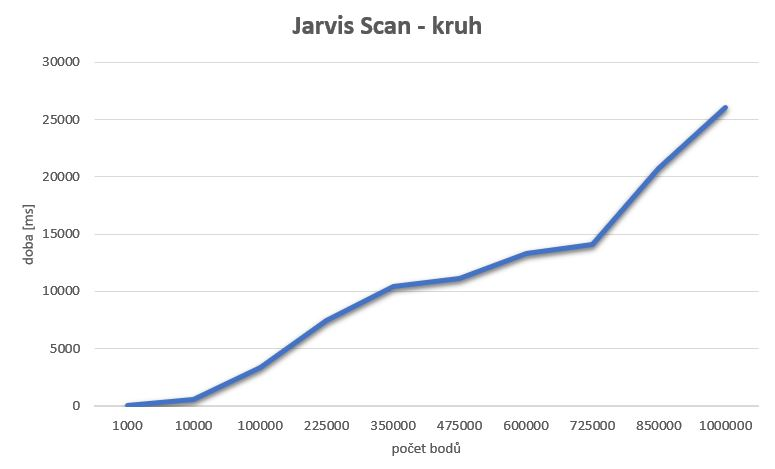
\includegraphics[width=10cm]{jarvis_kruh.jpg}
\end{figure}


\begin{figure}[h!]
	\centering
	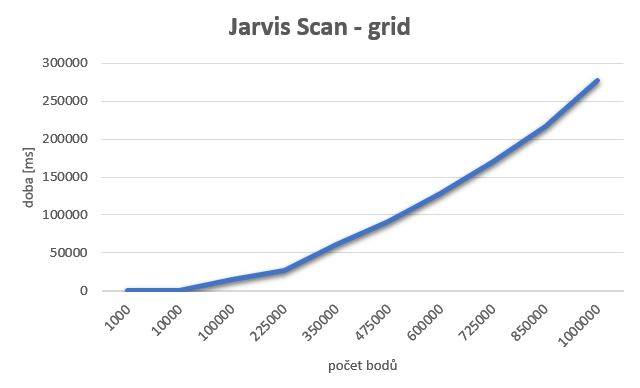
\includegraphics[width=10cm]{jarvis_grid.jpg}
\end{figure}


\begin{figure}[h!]
	\centering
	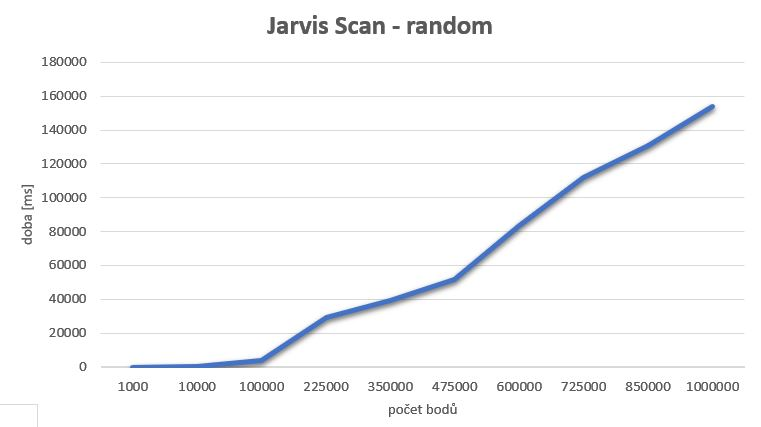
\includegraphics[width=10cm]{jarvis_random.jpg}
\end{figure}


\begin{figure}[h!]
	\centering
	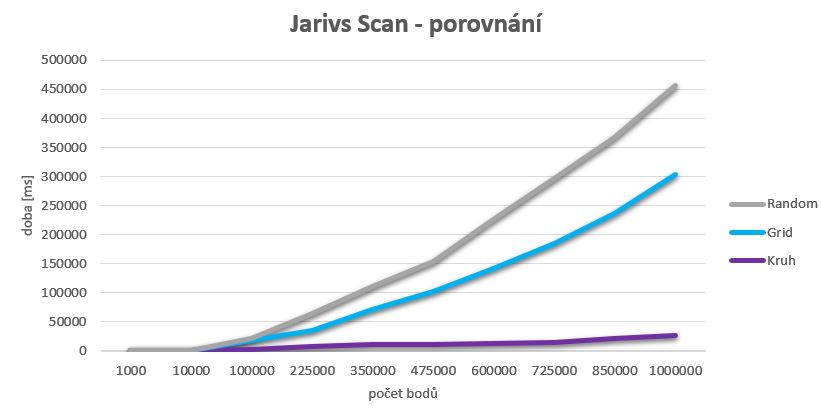
\includegraphics[width=10cm]{jarvis_vse.jpg}
\end{figure}

\clearpage


\subsection{Sweep Line}
Z dosavadních znalostí by tato metoda měla dosahovat velmi dobrých výsledků. Přesto v naší aplikaci dochází k chybě, při testování množiny bodů o 725.000 bodech začne aplikace pro náhodné rozmístění a kruh padat a je nefunkční. Na chybu se bohužel nepodařilo přijít.

\begin{figure}[h!]
	\centering
	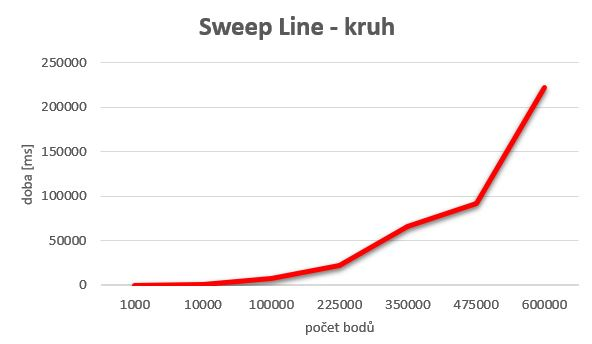
\includegraphics[width=10cm]{sweep_kruh.jpg}
\end{figure}


\begin{figure}[h!]
	\centering
	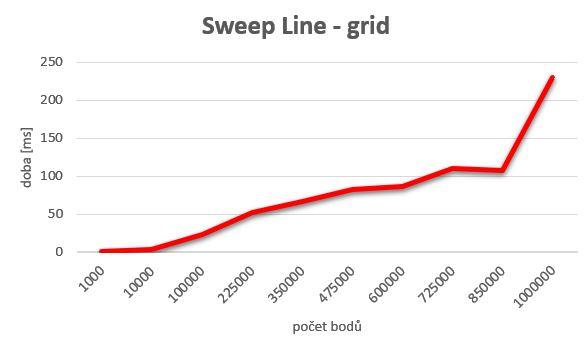
\includegraphics[width=10cm]{sweep_grid.jpg}
\end{figure}


\begin{figure}[h!]
	\centering
	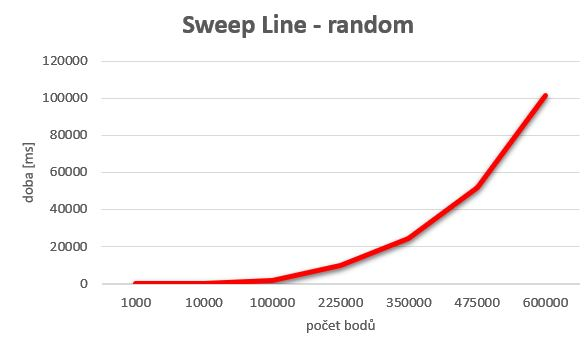
\includegraphics[width=10cm]{sweep_random.jpg}
\end{figure}
\clearpage

\subsection{Quick Hull}
Metoda Quick Hull dosahovala poměrně přiznivých výsledků. Velmi zajímavý byl graf porovnání výpočtu pro testované množiny, kde lze vidět, že funkce mají zhruba stejný průběh. Opět vychází nejlepší časy pro kruh a nejhorší pro náhodné rozmístění bodů.

\begin{figure}[h!]
	\centering
	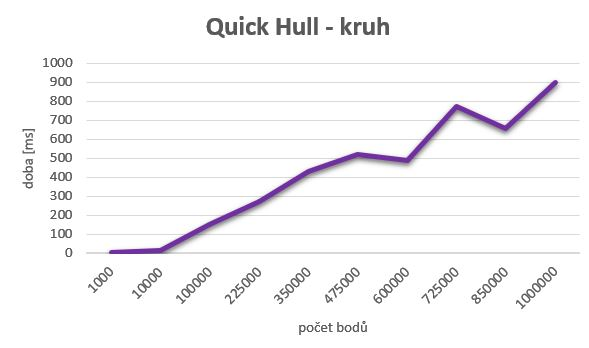
\includegraphics[width=10cm]{quickhull_kruh.jpg}
\end{figure}


\begin{figure}[h!]
	\centering
	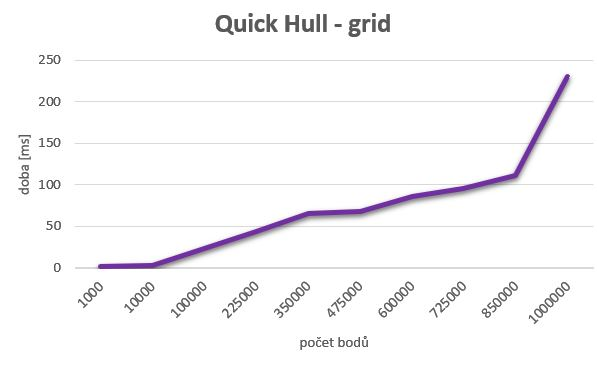
\includegraphics[width=10cm]{quickhull_grid.jpg}
\end{figure}


\begin{figure}[h!]
	\centering
	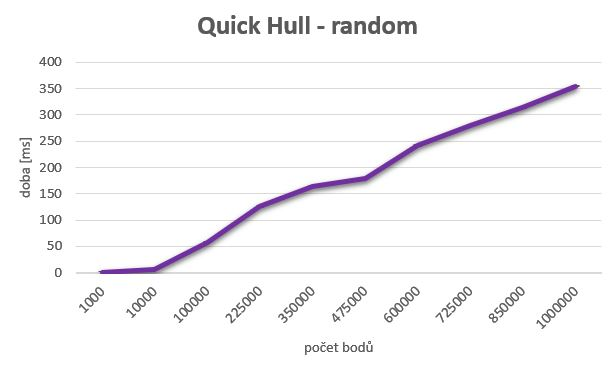
\includegraphics[width=10cm]{quickhull_random.jpg}
\end{figure}


\begin{figure}[h!]
	\centering
	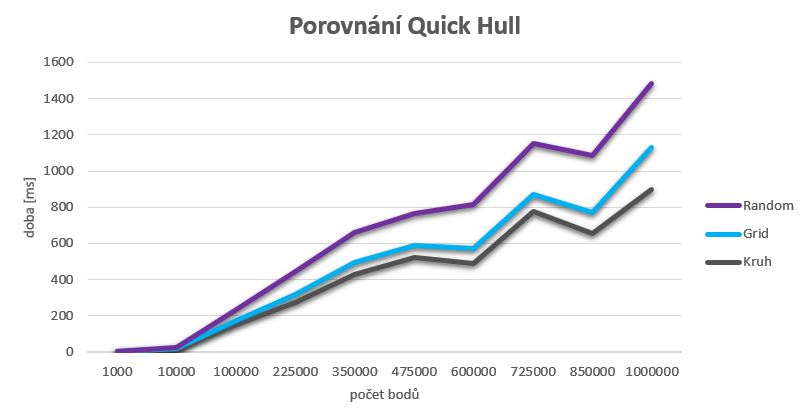
\includegraphics[width=10cm]{quickhull_vse.jpg}
\end{figure}


\subsection{Graham Scan}
Tento algoritmus dosahuje nejlepších výsledků. Metoda je rychlá a funkční. Pro kruh opět dosahuje nejlepších výsledků a nejhorších výsledků pro náhodné rozmístění bodů.

\begin{figure}[h!]
	\centering
	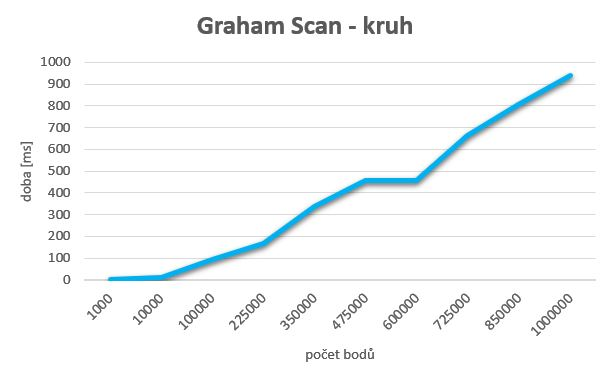
\includegraphics[width=10cm]{grahamscan_kruh.jpg}
\end{figure}


\begin{figure}[h!]
	\centering
	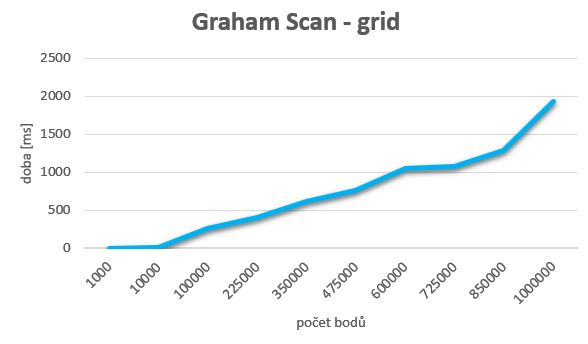
\includegraphics[width=10cm]{grahamscan_grid.jpg}
\end{figure}


\begin{figure}[h!]
	\centering
	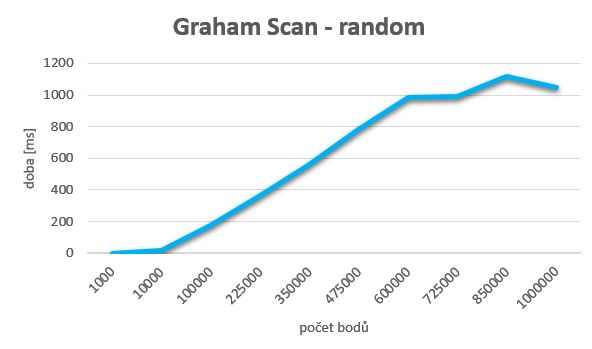
\includegraphics[width=10cm]{grahamscan_random.jpg}
\end{figure}


\begin{figure}[h!]
	\centering
	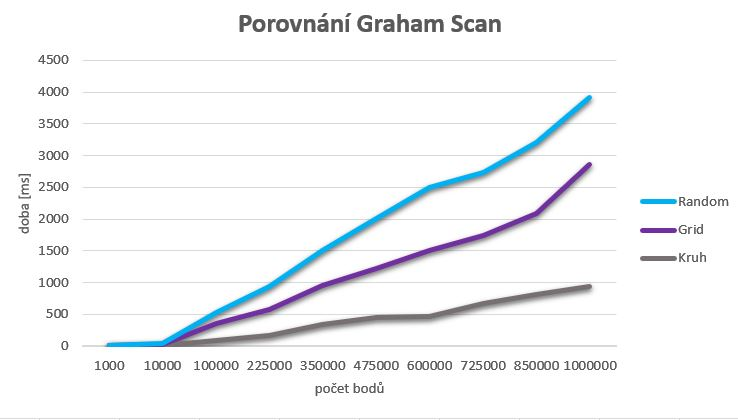
\includegraphics[width=10cm]{graham_vse.jpg}
\end{figure}



\clearpage
\subsection{Tabulky výsledných průměrných dob pro jednotlivé algoritmy}

Níže lze vidět tabulky s průměrnýmu naměřenými dobami jednotlivých algoritmů. Čas je uváděn v msec. První řádek vždy označuje počet bodů, druhý řádek množinu generovnou v kruhu, třetí řádek množinu v gridu a poslední řádek náhodné rozmístění bodů.


\begin{table}[h]
	\begin{tabular}{|r|r|r|r|r|r|r|r|r|r|}
	\hline
	  \textbf{1000} 	& \textbf{10000} & \textbf{100000} & \textbf{225000} & \textbf{350000} & \textbf{475000} & \textbf{600000}  & \textbf{725000}
 & \textbf{850000}  & \textbf{1000000}\\ \hline
			 76.2	& 603 	& 3323 & 7460 & 10409 & 11155 & 13280 &	14127 & 20775 & 26073 \\ \hline
	 32	& 893  	& 14664	& 27210 & 60533 & 91470 & 128758 & 170449 & 216169 & 276887 \\ \hline
	 11	& 191  	& 3562 & 29533 & 39542 & 51781 & 83605 & 112170 & 130838 & 153814	 \\ \hline

	
	\end{tabular}
		\caption{Jarvis Scan}
		
\end{table}


\begin{table}[h]
	\begin{tabular}{|r|r|r|r|r|r|r|r|r|r|r|}
	\hline
	 \textbf{1000} 	& \textbf{10000} & \textbf{100000} & \textbf{225000} & \textbf{350000} & \textbf{475000} & \textbf{600000}  & \textbf{725000}
 & \textbf{850000}  & \textbf{1000000}\\ \hline
	 1.8 & 15 & 151 &  273 & 430 & 520 & 487 & 774 & 657 & 898\\ \hline
	 1 & 3 & 23 & 43 & 65 & 68 & 86 & 96 & 112 & 231 \\ \hline
	 1 & 7 & 58 & 126 & 164 & 180 & 242 & 280 & 314 & 355	 \\ \hline

	
	\end{tabular}
		\caption{Quick Hull}
\end{table}






\begin{table}[h]
	\begin{tabular}{|r|r|r|r|r|r|r|r|r|r|r|}
	\hline
	 \textbf{1000} 	& \textbf{10000} & \textbf{100000} & \textbf{225000} & \textbf{350000} & \textbf{475000} & \textbf{600000}  & \textbf{725000}
 & \textbf{850000}  & \textbf{1000000}\\ \hline
	 1 & 115 & 7581 &  22199 & 65410 & 91985 & 222160 & - & - & -\\ \hline
	 1 & 4 & 23 & 52 & 67 & 83 & 87 & 110 & 108 & 230  \\ \hline
	2 & 35 & 1475 & 9938 & 24547 & 52011 & 101730 & - & -& -	 \\ \hline

	
	\end{tabular}
		\caption{Sweep Line}
\end{table}


\begin{table}[h]
	\begin{tabular}{|r|r|r|r|r|r|r|r|r|r|r|}
	\hline
	 \textbf{1000} 	& \textbf{10000} & \textbf{100000} & \textbf{225000} & \textbf{350000} & \textbf{475000} & \textbf{600000}  & \textbf{725000}
 & \textbf{850000}  & \textbf{1000000}\\ \hline
	 1.6  & 11 & 91 & 169 & 339 & 457 & 458 & 662 & 805 & 938   \\ \hline
	 1 & 16 & 256 & 406 & 611 & 763 & 1052 & 1081 & 1289 & 1926 \\ \hline
	 1 & 17 & 174 & 364 & 562 & 782 & 984 & 993 & 1117 & 1048 \\ \hline

	
	\end{tabular}
		\caption{Graham Scan}
\end{table}


\clearpage
\section{Závěr}
V rámci úlohy byla vytvořena aplikace, která je schopna na vygenerovaných bodech zkonstruovat konvexní obálku. Zároveň je v rámci aplikace možné náhodně vygenerovat téměř libovolné množství bodů do určitého tvaru. Na výběr je poměrně široké spektrum běžných tvarů, což jistě uživatel ocení.\\
\\
Součástí úlohy bylo i testování doby výpočtu jednotlivých konvexních obálek. Testování bylo prováděno nad striktně konvexními obálkami, samotný výpočet je tedy zatížen ještě o vyhodnocení, zda následující tři body neleží na stejné přímce. Výsledné doby dopadly dle očekávání. Algoritmus Jarvis Scan měl znatelně nejhorší čas. Naopak metoda Graham Scan se jeví jako nejlepší řešení.

\section{Náměty na vylepšení}
\subsection{Graham Scan}
Pro algoritmus Graham Scan byl nejprve napsán kod, který byl velmi náročný a aplikace nebyla funkční na větším množství dat. Z toho důvodu byla napsána nová metoda, která je již funkční a při testování dosahovala nejlepších možných výsledků. Z toho důvodu je v kódu pojmenována jako GrahamScanNew. Původní funkce byla v kódu ponechána pro případnou doeditaci a její zprovoznění.

\subsection{Generování množin bodů}
Při tvorbě generování gridu napadla autory myšlenka, že by se body generovaly v některém ze známých kartografických zobrazení. Z bakalářského studia znají velké množství zobrazovacích rovnic, pomocí nichž by se body zobrazovaly. Zajímavé rozmístění by měla zejména kuželová zobrazení. Při zobrazení bodů v rámci některého kartografického zobrazení by výsledná konvexní obálka představovala celý svět, případně polokouli, záleželo by na typu zvoleného zobrazení.

\subsection{Testování algoritmů}
V rámci této úlohy bylo provedeno několik testování nad odlišným množstvím bodů a na jejich odlišném zobrazení. Časově bylo testování poměrně náročné, za úvahu jistě stojí popřemýšlení, zda by nebylo výhodnější vytvořit takovou funkci, která by pro předem definované tvary a množství bodů sama provedla testování. Zároveň obsahuje platforma Qt i knihovnu grafů, časová úspora by tedy byla velmi výrazná.


\subsection{Tvorba tabulek v LaTeXu}
V rámci dokumentace bylo i prezentování výsledných měření prostřednictvým tabulek. V původních tabulkách byl ještě sloupec, který označoval typy množin (kruh, grid, random). Bohužel s tímto sloupcem byla tabulka oříznutá a přes veškerou snahu se autorům nepodařilo nalézt řešení, jakým způsobem tabulku posunout vlevo. Z toho důvodu byl tento sloupec odstraněn a tabulky byly popsány v záhlaví podkapitoly. S tímto řešením nejsou autoři zcela spokojeni, tabulky nejsou dostatečně přehledné. 

\subsection{Minimum Area Enclosing Box}
Při výpočtu minimálního ohraničujícího obdélníku autorům z neznámé příčiny nefungovala transformace, ač se to snažili vyřešit. Po konzultaci byla část pro transformaci vypůjčena od kolegy, kterému fungovala bez problémů. Vypůjčená část je v kódu vyznačena. 





\clearpage
\section{Reference}

\begin{enumerate}
\item  MARTÍNEK, Petr. Konvexní obálka rozsáhlé množiny bodů v E\^d [online][cit. 31.10.2018]. \\
Dostupné z: http://graphics.zcu.cz/files/86\_BP\_2010\_Martinek\_Petr.pdf  \\

\item Convex Hulls: Explained. [online][cit. 31.10.2018]\\
Dostupné z: https://medium.com/@harshitsikchi/convex-hulls-explained-baab662c4e94\\

\item Convex-hull mass estimates of the dodo (Raphus cucullatus). [online][cit. 31.10.2018]\\
Dostupné z: https://www.semanticscholar.org/paper/Convex-hull-mass-estimates-of-the-dodo-(Raphus-of-a-Brassey-O\'Mahoney/12e07d3b712561cad16501ac8096120e14901eb8

\item GeeksforGeeks: Convex Hull - Set 1 (Jarvis's Algorithm or Wrapping. [online][cit. 5.11.2018]\\
Dostupné z: https://www.geeksforgeeks.org/convex-hull-set-1-jarviss-algorithm-or-wrapping/

\item  BAYER, Tomáš. Geometrické vyhledávání [online][cit. 5.11.2018]. \\
Dostupné z: https://web.natur.cuni.cz/~bayertom/images/courses/Adk/adk4.pdf  \\

\item GeeksforGeeks: Convex Hull - Set 2 (Graham Scan). [online][cit. 12.11.2018]\\
Dostupné z: https://www.geeksforgeeks.org/convex-hull-set-2-graham-scan/



\end{enumerate}
\end{document}



 